\documentclass[twoside,bibliography=totoc,openany]{fumi}

% Definition von Variablen
\newcommand{\thesistitle}{Template für Abschlussarbeiten v0.1}
\newcommand{\thesisauthor}{Maxi Musterfrau}
\newcommand{\thesistype}{Masterarbeit} % Bachelorarbeit, Diplom, Masterarbeit, ects.
\newcommand{\thesismatrikelnummer}{01234567}

% Tell LaTeX about how to wrap words using the correct german hyphenation rules.
\hyphenation{Lern-arrange-ments Lern-arrange-ment Lern-aktivität Lern-aktivitäten doku-mentiert Hash-funk-tion Hash-funk-tionen Video-frames Video-frame Link-ak-ti-vier-ung Co-decs Link-ob-jekt-es  Hyper-video-Autoren-um-geb-ung-en  App-li-kat-ion-en  Kon-tain-er-for-mat Bild da-tei-en  Co-decs Brow-ser   Au-to-ren-um-ge-bun-gen Aus-zeich-nungs-spra-che spe-zi-fische Vi-deo-lern-um-ge-bung-en Vi-deo-lern-um-ge-bung Lern-um-ge-bung Lern-um-ge-bung-en}

\title{\thesistitle}
\author{\thesisauthor}
\date{\today}


%%%%%%%%%%%%%%%%%%%%%%
\begin{document}
\sffamily
\pagestyle{empty}


%% Titelseite (optional für die PDF-Version des Textes)
%\includepdf[pages=-, offset=0 0]{img/cover.pdf}\newpage~\newpage

%% Die erste Seite eines Buches
\thesisauthor\\{\textbf{\thesistitle}}\vfill\newpage~\newpage

%% Die Seite mit den Titelangaben
\vspace{2cm}
\begin{center}\LARGE
\vfill
{\Huge\thesistitle}\\
\vfill
\thesistype\\
\vfill
eingereicht von\\[4pt]
\textbf{\thesisauthor}\\[4pt]
(Matrikelnummer \thesismatrikelnummer)\\
\vfill
angefertigt am\\
Lehrgebiet Kooperative Systeme\\
Fakultät Mathematik und Informatik\\
FernUniversität in Hagen\\
\vfill 
Betreuer\\
Dr. Niels Seidel
\vfill
\monthname[\the\month] \the\year
\end{center}
\newpage~\newpage

%% Leerseite mit Titel
{\large\textbf{\thesisauthor}\\\textbf{\thesistitle}\vfill}\newpage~\newpage


%% Seite mit Zusammenfassung und englishsprachigen Summary
\section*{Zusammenfassung}
\dots\vfill
\section*{Summary}
\dots\vfill\newpage

%% Seite mit bibliografischen Angaben
{\small
%Herausgeber: Namen der Herausgeber\\

% Zitation
\thesisauthor. \textit{\thesistitle}. \thesistype. Fakultät Mathematik und Informatik, FernUniversität in Hagen, \the\year. %\href{}{}. % optional URN
\\\vfill

% Optional, jedoch sehr zu empfehlen
Diese Publikation ist unter \emph{Creative Commons -- Namensnennung 3.0 Deutschland} lizenziert und darf als Ganzes oder ausschnittweise vervielfältigt, verbreitet und öffentlich zugänglich gemacht werden, sofern dies im Text nicht anders vermerkt ist.\newline\vspace{10pt}
\hspace{-9pt}
\includegraphics[height=10mm]{logo-cc.pdf}
\\\vspace{10pt}

% ISBN: \dots\\
% URN: \href{...}
Autor: \thesisauthor\\
Gestaltung und Satz: \thesisauthor / \LaTeX\\
% Lektorat: Claudia Neumann\\ optional
% Titelbild: \dots\\optional
Datum: \today\\
% Printed in Germany
\cleardoublepage
}

%% Inhaltsverzeichnis
\pagestyle{headings}
\tableofcontents


%%%%%%%%%%%%%%%%%%%%%%%%%%%%%%%%%%%%%%%%%%%%%%%%%%%
\chapter{Ein einleitendes Kapitel}

%%%%%%%%%%
\section{Einleitung}
Dieses Dokument dient als Vorlage für Abschlussarbeiten, die mit Hilfe von \LaTeX geschrieben und gesetzt werden. Es erfüllt somit weniger den Zweck Ihnen eine Einführung in \LaTeX zu geben, als die Richtwerte für Satz und Layout festzulegen. 

Um das Dokument $main.tex$ in ein PDF zu verwandeln, müssen Sie \texttt{pdflatex} verwenden und folgenden Befehl ausführen: \texttt{pdflatex main}. 


%%%%%%%%%
\section{Seitenlayout}

Eine Seite hat das Format A4 mit den Abmessungen 210\,mm in der Breite und 297\,mm in der Höhe. Der obere und unter Rand misst 3\,cm. Der innere und äußere Rand beträgt 2\,cm. Die Seiten Zahlen erscheinen auf ungeraden Seiten rechts unten und auf geradzahligen Seiten links unten auf einer Seite. In der Kopfzeile erscheint auf den geradzahligen Seiten das Kapitel (z.B. \textquote{Kapitel 1: Einführung}) und auf den ungeradzahligen Seiten der jeweilige Abschnitt (z.B. \textquote{1.2 Seitenlayout}). Eine Ausnahme davon stellt die erste Seite eines Kapitels dar, auf denen die Kopfzeile leer bleibt. Zu beachten ist, dass neue Kapitel stets auf einer ungeraden Seite, rechts im zweiseitigen Layout eines Buches beginnen. 
%	footskip={15mm},
%	headheight={20mm}


%%%%%%%%%
\section{Text und Überschriften}
Die Schriftgröße beträgt 11\,pt. Innerhalb des Textes gibt es keinen Grund, davon abzuweichen. Als Schriftart sollten Sie versuchen Schriften aus der Familie \textit{Frutiger} bzw. ähnliche Schriftarten\footnote{Siehe \url{https://de.wikipedia.org/wiki/Frutiger} sowie \url{http://joelcrawfordsmith.com/closest-font/font/frutiger} (abgerufen am 06.06.2018).}, notfalls jedoch Arial zu verwenden. %Diese, leider lizenzpflichtigen Schriftarten können Sie als Studierende kostenlos von der FernUniversität beziehen: \url{https://www.fernuni-hagen.de/zmi/download/#frutiger} (abgerufen am 13.05.2018).

Hervorhebungen im Text sollten nur kursiv (\verb|\textit{}|) und nur in seltenen Ausnahmen fett\linebreak (\verb|\textbf{}|) kenntlich gemacht werden. 

Hyperlinks sollten innerhalb eines PDFs benutzbar sein. Nutzen Sie dazu den Befehl \verb|\url{}|. Hinter einer jeden URL sollten Sie in Klammern das Datum des letzten Abrufs angeben.

Querverweise auf Abbildungen, Tabellen und Abschnitte können Sie mit dem Befehl \verb|\ref{}| erzeugen, sofern beim Verweisziel eine \verb|\label{}| mit identischem Bezeichner definiert wurde (z.B. \verb|\label{Querverweise}| und \verb|\ref{Querverweis}|). Sollte sich das Verweisziel mehr als zwei Seiten entfernt liegen, sollte auch die Seitenzahl mit angegeben werden:\\ 
\verb|siehe Abschnitt \textit{Querverweis} (S.~\pageref{Querverweis})|\\ bzw. 
\verb|(Abschn. \textit{Querverweis}, S.~\pageref{Querverweis})|

Die Hierarchie von Überschriften beginnt bei Kapiteln (\verb|\chapter{}|, 20\,pt) und geht über Abschnitte (\verb|\section{}|, 14\,pt), Teilabschnitte (\verb|\subsection{}|) bis hin zu \verb|\subsubsections{}| und \verb|\paragraph{}|. Letztere beide sollten aus Gründen der Übersichtlichkeit nicht im Inhaltsverzeichnis erscheinen.

Zeilenumbrüche nimmt LaTeX in der Regel automatisch vor. Dennoch kommt es zu sehr unschönen Trennungen von deutschsprachigen Wörtern (z.B. Ei-nkaufen) oder Überschreitungen des Seitenrands. Um LaTeX bevorzugte Worttrennungen vorzuschlagen können Sie diese entweder direkt innerhalb eines Wortes vermerken (\verb|Ein\-kaufen|) oder bei häufigeren Vorkommen am Beginn des Dokumenten vermerken: \verb|\hyphenation{Ein-kauf.en Ein-kreis-en}|. Gewünschte Zeilenumbrüche lassen sich mit \verb|\linebreack| und erzwungene Umbrüche mit \verb|\newline| erzeugen. 

Die Verbindung von Zahlen und Maßeinheiten wird durch ein halbes Leerzeichen getrennt (\verb|\,|). Beachten Sie den Unterschied zwischen \textquote{30m weit}, \textquote{30 m weit} und der korrekten Darstellung \textquote{30\,m weit}.

Ligaturen wie fi, L-S sollten Sie nicht als Darstellungsfehler, sondern als typografische Besonderheit verstehen.

%%%%%%%%%
\section{Tabellen}
Für Tabellen empfiehlt sich die Umgebung \textit{tabularx}, um einerseits die Breite der gesamten Tabelle und andererseits gleichmäßig breite Spalten zu erhalten: \verb|\begin{tabularx}{\textwidth}{lrrX}|
Die Textausrichtung je Spalte wird durch die Parameter l, r, X, L oder R definiert.

Beachten Sie bei Tab.~\ref{Tabellenbeispiel} den sparsamen Einsatz von Rahmungen sowie Spalten- und Zeilenumrandungen. Um Zeilen voneinander abzugrenzen können Sie den Abstand der Tabellenzeilen definieren (z.B. \verb|\def\arraystretch{1.4}|).
Auch die Hervorhebung der Kopfzeilen ist nicht notwendig. Beachten Sie Tabellen stets mit einer Überschrift zu versehen, die im Gegensatz zu Bildunterschriften auch oberhalb der Tabelle platziert wird.

\begin{table}[!ht]
\def\arraystretch{1.4}
\label{Tabellenbeispiel}
\caption{Eine Tabelle mit Inhalt}
 \begin{tabularx}{\textwidth}{lrrX}      
    \hline
    Day & Min Temp & Max Temp & Summary 
    \\\hline
    Monday & 11\,C & 22\,C & A clear day with lots of sunshine.
    However, the strong breeze will bring down the temperatures. \\
    Tuesday & 9\,C & 19\,C & Cloudy with rain, across many northern regions. Clear spells 
    across most of Scotland and Northern Ireland, 
    but rain reaching the far northwest. \\
    Wednesday & 10\,C & 21\,C & Rain will still linger for the morning. 
    Conditions will improve by early afternoon and continue 
    throughout the evening. \\
    \hline
    \end{tabularx}
\end{table}
%\clearpage

%\addcontentsline{lot}{table}{Tabelle}
%\paragraph{Kommentare zur Tabelle:}
%$\{$lr|c$\}$ bedeutet, dass die erste Spalte linksbündig, die zweite
%Spalte rechtsbündig, dann eine Linie und die dritte Spalte zentriert
%gesetzt wird.


\section{Abbildungen}

Die Abb.~\ref{einbild} zeigt ein Foto einer Lehrveranstaltung, welches im PNG-Format vorliegt. Selbst gezeichnete Abbildungen (siehe Abb. \ref{nocheinbild}) sollten als skalierbare Grafiken (z.B. als PDF oder EPS) eingebunden werden, um eine responsive Darstellung zu erhalten. Zudem kann LaTeX PDFs schneller einbinden, als typische Bildformate.

\begin{figure}[h!]

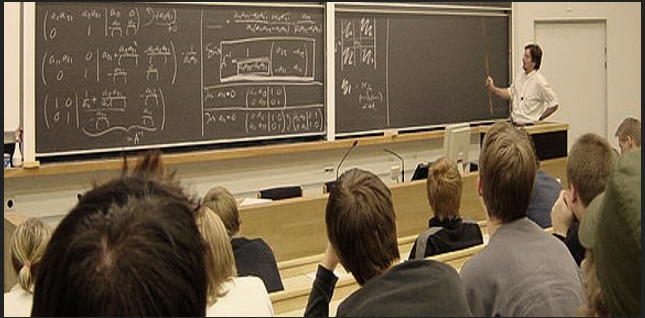
\includegraphics[width=\textwidth,left]{figure.png}
\caption{\label{einbild}Eine realistische Abbildung als PNG-Datei}
\end{figure}

\begin{figure}[h!]
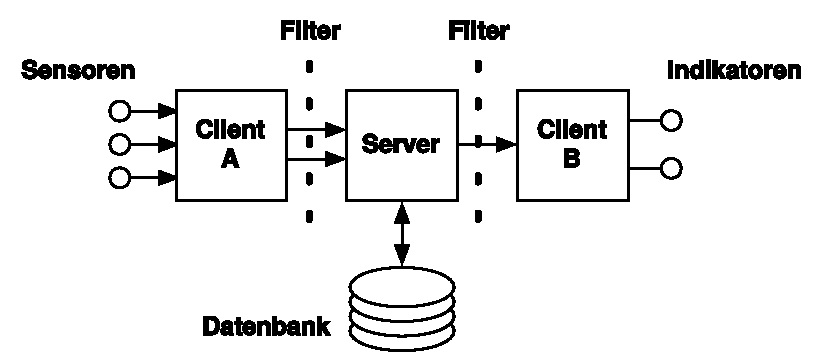
\includegraphics[width=\textwidth,left]{figure2.pdf}
\caption{\label{nocheinbild}Eine mit \textit{InkScape} selbst gezeichnete Abbildung, die als PDF eingebunden wurde.}
\end{figure}
\clearpage

%%%%%%%%
\section{Mathematische Ausdrücke}

Mathematische Ausdrücke können Sie innerhalb einer Zeile (z.B. $\text{ID} = \log_2 \frac{2D}{W}$, ausgeschrieben im Code: \verb|$\text{ID} = \log_2 \frac{2D}{W}$|) oder in einem gesonderten Absatz darstellen:
\begin{formel}[!ht]
   \begin{equation}
     \text{ID} = \log_2 \Bigg(\frac{2D} {W}\Bigg)
   \end{equation}
   \caption{Fitts's Law als Beispiel für eine Formel.}
\end{formel}



%%%%%%%%
\section{Quellcode und Pseudocode}
Im Quelltext dieses Abschnitts finden Sie das nachfolgende Code-Beispiel (\ref{meinlisting}) sowie den exemplarischen Algorithmus (ref{algo})


\begin{lstlisting}[basicstyle=\small,
             inputencoding={utf8}, 
             extendedchars=false,
             commentstyle=\color{black}, 
             keywordstyle=\color{black}, 
             escapeinside=``,
             linewidth=.99\textwidth,
             caption={Eine kurze Codesequenz},
             label={listing:meinlisting}]
t=npt:<start-in-seconds>,<end-in-seconds>
t=npt:<m>,<s>.<ms>:<h>:<m>.<ms>
t=smpte-<frame-rate>:<h>:<m>:<s>,<h>:<m>:<s>.<ms>
\end{lstlisting}

\scalebox{.8}{ 
\begin{algorithm}[H]
\caption{\label{algo}Ein exemplarischer Algorithmus}

\KwIn{~\\
$ Log $: Clickstream log\\
$\varepsilon$ Tolerance 
}
~\\
\SetKwFunction{getUserPlaybackTime}{getUserPlaybackTime}
\SetKwProg{myalg}{Function}{}{End}
  \myalg{\getUserPlaybackTime{userSessionLog}}{
  	$tmp\gets userSessionLog[0]$\\
	\For{$i=1;  i < length(userSessionLog); i\gets i+1$}{
		$timeDistance\gets userSessionLog[i].utc - tmp.utc$\\
		$playbackDistance\gets userSessionLog[i].playbacktime - tmp.playbacktime$\\
		\If{$ playbackDistance > 0$}{
			\If {$ (timeDistance - playbackDistance)  \le \varepsilon $~}{
				   $playbackTime\gets playbackTime + playbackDistance$
			}
		}
		$tmp\gets Log[i]$
	}
\KwRet $playbackTime$}{}
\end{algorithm} 
 }
 

%%%%%%%%
\section{Literaturverweise und Fußnoten}
Um auf eine Literaturstelle verweisen zu können sollten Sie sich mit BibTex oder Biblatex auseinandersetzen. In diesem Formaten sind die Literaturangaben je Publikationsart (z.B. Buch, Buchbeitrag, Konferenz- oder Journalbeitrag) notiert. 

Mit dem  Befehl \verb|\bibliography{/pfad/zu/meiner/bibtext-datei}| geben Sie den Pfad zu Ihrer BibTex Bibliografie an. In Mendeley können Sie beispielsweise eine solche Datei an einem bestimmten Ort ablegen und automatisch aktuell halten.

Zur Verwaltung von Bibliografien verwenden wir \textit{Natbib}. Um damit ein Werk passiv zu zitieren nutzt man den Befehl \verb|\citep{}|. Aktive Zitation, bei denen die Namen der Autoren, gefolgt vom Erscheinungsjahr in Klammern erscheinen, schreiben Sie \verb|\citet{}|. Siehe dazu Tab.~\ref{zitiercmd}. In die geschweiften Klammern fügen Sie jeweils den gewünschten Zitationsschlüssel aus der BibTex oder Biber Datei ein. 

Als Zitierstil wird APA empfohlen, da im Text sowohl die Autoren, als auch das Erscheinungsjahr unmittelbar nachvollzogen werden kann. Genauere Informationen zur korrekten Zitierweise finden Sie unter \url{http://www.apastyle.org/} (abgerufen am 13.05.2018).

Fußnoten dienen nicht zur Angabe von Zitationen. Sie können jedoch genutzt werden, um dem Leser zusätzliche Informationen zu vermitteln, die ansonsten den Lesefluss des Haupttextes stören würden (z.B. URLs\footnote{Siehe \url{https:\\example.com/} (abgerufen am 13.05.2018).}).

\begin{table}\footnotesize
\caption{\label{zitiercmd}Zitation von Literatur}
\begin{tabularx}{\textwidth}{lXX}
\hline
Befehl & Beispiel & Beschreibung\\\hline
\verb|\citet{}| & \citet{Guerra-Hollstein2017} & Aktive Zitierweise\\
\verb|\citep{}| & \citep{Guerra-Hollstein2017} & Passive Zitierweise\\
\verb|\citet*{}| & \citet*{Guerra-Hollstein2017} & Wie \verb|\citet|, wobei all Autoren genannt werden\\
%\citep*{Guerra-Hollstein2017} & Wie \verb|\citep|, wobei all Autoren genannt werden\\ 
\verb|\citeauthor{}| & \citeauthor{Guerra-Hollstein2017} & Gibt nur die Namen der Autoren aus\\
\verb|\citeyear| & \citeyear{Guerra-Hollstein2017} & Gibt nur das Erscheinungsjahr aus\\
\hline
\end{tabularx}
\end{table}

%%%%%%%%
\section{Sonstiges}

\todo[inline]{Im Bearbeitungsprozess möchte man dem Leser manchmal etwas mitteilen, was nicht im Text stehen soll.} Dafür eignet sich das todo-Packet mit dem Befehl \protect\verb|\todo[inline]{}|. {\color{red} Sie können solche Informationen natürlich in einer anderen Farbe hinterlegen (\verb|{\color{red} \dots}|).}

Definitionen: \verb|\begin{definition}\dots\end{definition}|

\begin{definition}
Eine Abschlussarbeit ist international eine wissenschaftliche oder künstlerische Arbeit, die für den Abschluss eines Masterstudiengangs verfasst wird.
\end{definition}

Kommentare im Quelltext werden im PDF nicht angezeigt:\\ Definitionen: \verb|\begin{comment}\dots\end{comment}|


%%%%%%%%%%%%%%%%
\chapter{Ein weiteres Kapitel}
%% lade Kapitel aus Datei
\dots
Text aus dem zweiten Kapitel
\dots




%%%%%%%%%%%%%%%% ANHANG
\appendix

%%
\chapter{Erster Teil des Anhangs}
\dots

%%
\chapter{Zweiter Teil des Anhangs}
\dots




%%% Verzeichnisse
\backmatter
\pagestyle{fancyclear}



%% Literaturverzeichnis
%\phantomsection\addcontentsline{toc}{chapter}{Literaturverzeichnis}
{\footnotesize\flushleft\setlength{\itemsep}{-3pt}%\setlength{\bibsep}{3pt}
\bibliographystyle{plainnat}
\bibliography{/home/abb/Documents/library}}
\cleardoublepage


%% Abbildungsverzeichnis
\phantomsection\addcontentsline{toc}{chapter}{Abbildungsverzeichnis}
\listoffigures
\cleardoublepage


%% Tabellenverzeichnis
\phantomsection\addcontentsline{toc}{chapter}{Tabellenverzeichnis}
\listoftables
\cleardoublepage


%% Auflistungsverzeichnis
\phantomsection\addcontentsline{toc}{chapter}{Auflistungsverzeichnis}
\renewcommand\lstlistlistingname{Verzeichnis der Auflistungen}
\lstlistoflistings
\cleardoublepage


%% Verzeichnis von Algorithmen
\phantomsection\addcontentsline{toc}{chapter}{Verzeichnis der Algorithmen}
\renewcommand*\listalgorithmcfname{Verzeichnis der Algorithmen}
\listofalgorithms
\cleardoublepage


%% Abkürzungsverzeichnis
\phantomsection\addcontentsline{toc}{chapter}{Abkürzungsverzeichnis}
\chapter*{Abkürzungsverzeichnis}

\begin{description}
\item[AICC] Aviation Industry Computer-Based Training Committee
\item[AJAX] Asynchronous JavaScript and XML
\item[API] Application Programing Interface
\item[BMBF] Bundesministerium für Bildung und Forschung
\end{description}
\cleardoublepage


%% Erklärung ...
Name: \thesisauthor \hfill Matrikelnummer: \thesismatrikelnummer \vspace{2cm}
\subsection*{Eidesstattliche Erklärung}
Ich erkläre hiermit, dass ich diese \thesistype~selbständig verfasst, noch nicht anderweitig für Prüfungszwecke vorgelegt, keine anderen als die angegebenen Quellen und Hilfsmittel benutzt sowie wörtliche und sinngemäße Zitate als solche gekennzeichnet habe.\\[1cm]
Hagen, den \dotfill

\hspace{2cm}{\footnotesize Datum}\hspace{5cm} {\footnotesize \thesisauthor}



\end{document}
